\chapter{J/$\Psi$ Transverse Spin Dependent Analysis}
\label{ch::jpsi}
\ifpdf
\graphicspath{{Chapters/JPsi/Figs/}}
\fi

This chapter describes the analysis performed in the intermediate invariant mass
range at COMPASS.  The biggest advantage about the intermediate mass range is an
increase in statistics.  The intermediate mass range contains 1.6 times more
data than the high mass range about 4.3~{\gvcw}.  On the other hand, the
intermediate mass range results from several reactions.  By far the most
dominate reaction is {\jp} production.  A theoretical introduction related to
transverse {\jp} spin asymmetries is provided in Sec~\ref{sec::theory_jpsi}.  As
of yet however, the exact mechanism for J/$\Psi$ production is unknown and
therefore the exact {\jp} vertex coupling is unknown.  Never the less, the
analysis techniques in this chapter contributes to the transverse spin knowledge
from J/$\Psi$ production.  The reaction of interest is
\begin{equation}
  \pi^-(P_a) + P(P_b, S_T) \rightarrow J/\Psi + X \rightarrow \mu^-(\ell) +
  \mu^+(\ell') + X,
\end{equation}
\noindent
where the proton target, $P$, is transversely polarized with spin $S_T$.

The dimuon final state from {\jp} production is indistinguishable from the
Drell-Yan dimuon final state described the previous analyses in
chapter~\ref{ch:hmanalysis}.  For this reason, similar event selection and data
quality are used to study the dimuon production resulting from {\jp} decays.  On
the other hand, the {\jp} production has a higher background percentage from
Drell-Yan and other components to be taken into account.  The results presented
in this chapter are determined from the left-right asymmetry analysis as in
Sec~\ref{sec::leftrightasym}, where again the left-right asymmetry is defined as

\begin{equation}
  A_{lr} = \frac{1}{|S_T|}
  \frac{\sigma_l - \sigma_r}{\sigma_l +
    \sigma_r}.
\end{equation}

\subsection{Data Collection and Event Selection}
The data collection is described in Sec~\ref{sec:datacollection} and the data
stability tests are described in Sec~\ref{stability}.  Both the Drell-Yan
analysis and the {\jp} production analysis study dimuon final states so the
spectrometer data taking conditions are the same.  In particular the measurement
in this chapter results from a 190~{\gvc} $\pi^-$ beam impinged on a
transversely polarized NH$_3$ target from the 2015 COMPASS spectrometer data
taking conditions.

The event selection in this chapter is similar to the event selection in the
previous chapter, Sec~\ref{sec::dy_eventselection}.  The cuts are chosen to
ensure two oppositely polarized muons are detected with a vertex in the
transversely polarized NH$_3$ target.  Table~\ref{tab::cutdescrip} describes the
cut selection and the reason from each cut.  The only event selection
difference, from Table~\ref{tab::cutdescrip}, is the selected invariant mass.
The nominal {\jp} invariant mass and width are 3.096~{\gvcw} and
92.9$\times10^{-6}$~{\gvcw} respectively~\cite{Tanabashi:2018oca}.  Therefore to
ensure the events for this analysis result from {\jp} production, the analysis
invariant mass range should be where {\jp} signal to background is highest.
This is in contrast to the Drell-Yan analyses which require the invariant mass
to be above 4.3~{\gvcw}.

\subsubsection{{\jp} Invariant Mass Range}
The COMPASS spectrometer has a finite mass resolution which therefore means the
events resulting from {\jp} production have an invariant mass spread larger than
the nominal {\jp} width.  For this reason the cut on invariant mass should be a
range much larger than the nominal {\jp} width.
Fig.~\ref{fig::DY_InvariantMassJPsi} shows the 2015 dimuon invariant mass
distribution and the other production components around the {\jp} invariant
mass.

\begin{figure}[h!t]
  \centering 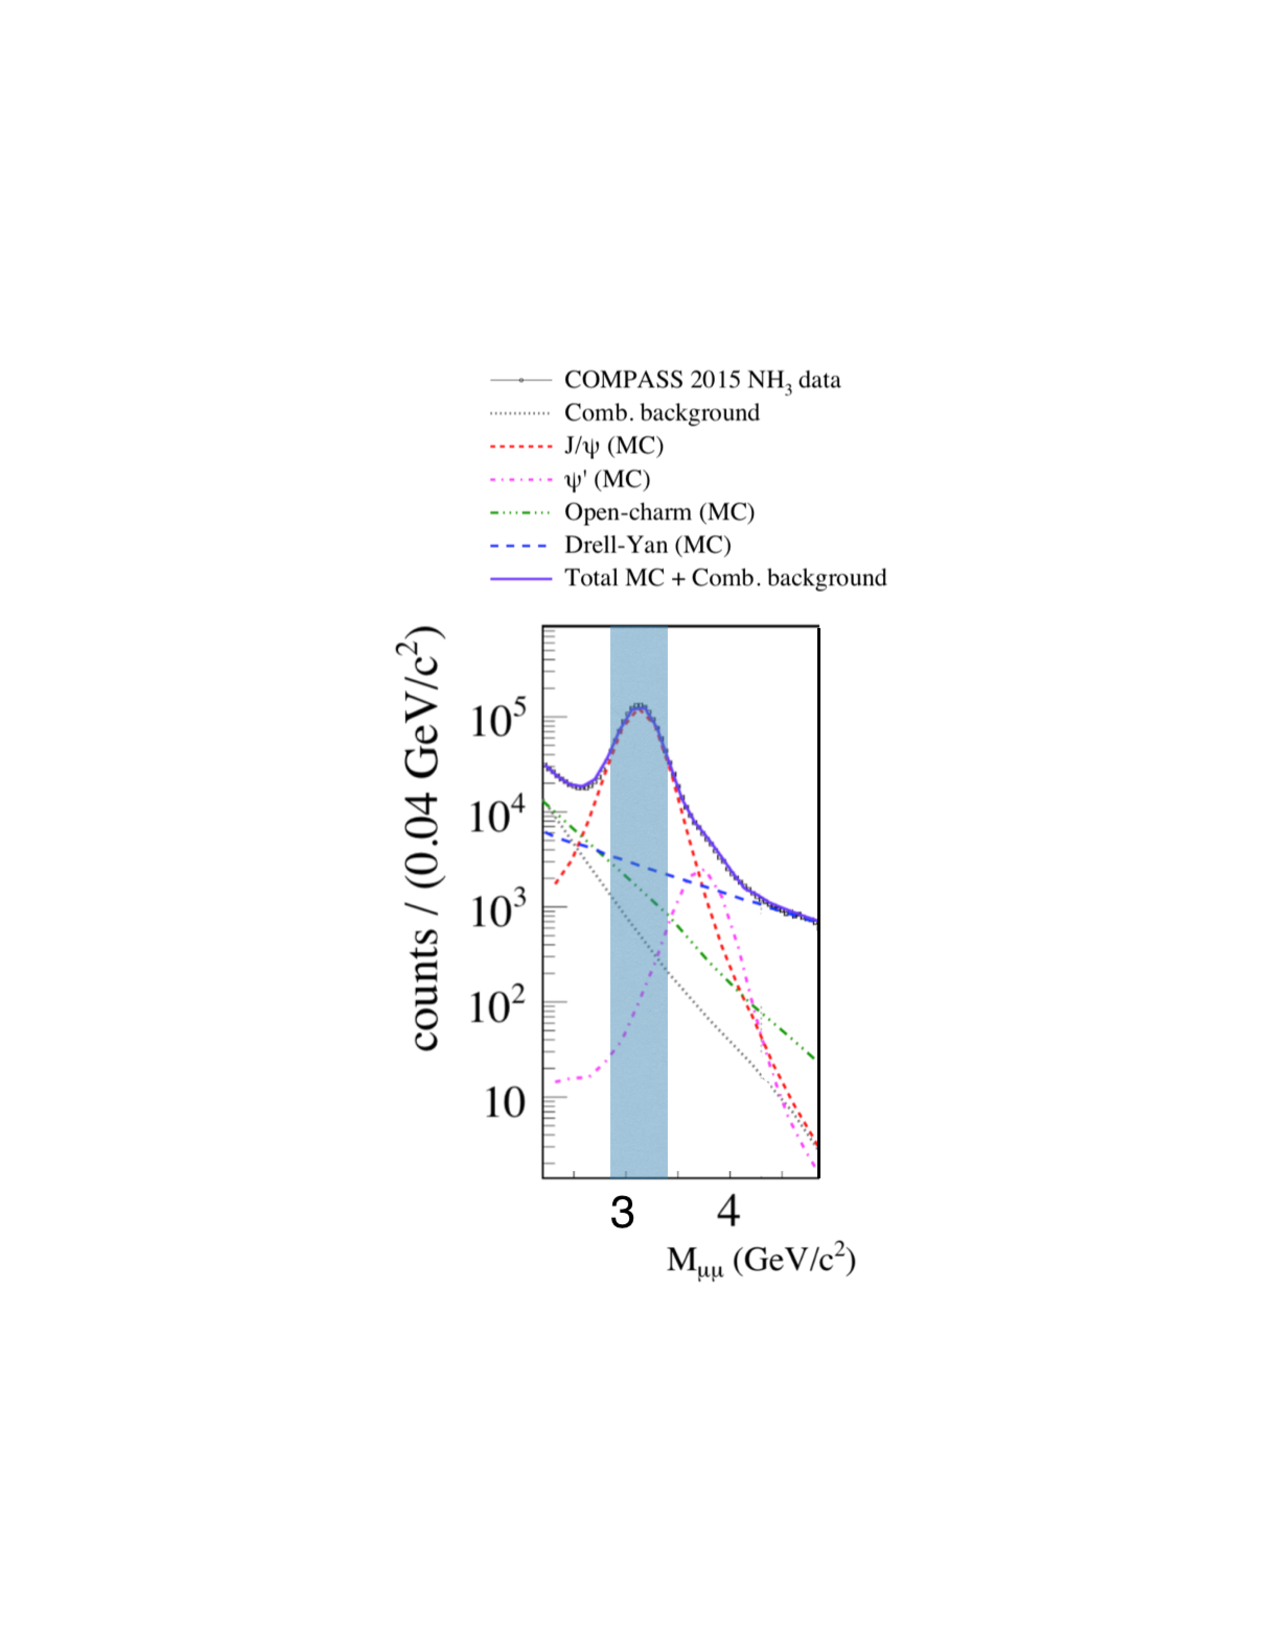
\includegraphics[width=0.3\textwidth,trim=6cm 6cm 6cm 5.5cm,
    clip]{DY_InvariantMassJPsi}
  \caption{The 2015 COMPASS invariant dimuon mass distribution and a fit to this
    data.  The data fit is from Monte-Carlo and combinatorial background
    analysis and is provided to show the background processes.  This image is
    taken from~\cite{compassDYpaper}.}
  \label{fig::DY_InvariantMassJPsi}
\end{figure}

As can be seen in Fig.~\ref{fig::DY_InvariantMassJPsi}, regardless of the
analysis mass range chosen, there are still events resulting from the other
background processes.  The normalized systematic variance resulting from
background processes is derived in Appendix~\ref{app::sysEventContam} as

\begin{equation}
  \frac{\sigma^2_{systematic}}{\sigma^2_{statistical}} = \frac{(1-p)^2}{p^2},
\end{equation}
\noindent
and the total variance from statistical fluctuations and background
contributions is
\begin{equation}
  \delta^2 A_{lr,J/\Psi} = \frac{(1-p)^2 + 1}{p^2}\sigma^2_{statistical},
  \label{equ::JPerrorTot}
\end{equation}
where $p$ is the {\jp} purity.  Therefore the analysis invariant mass range
should have a {\jp} purity as high as possible to reduce the systematic error
while still including as much data as possible to reduce the statistical error.
The total error however, is dominated by statistical error for any purity larger
than 50\%.  That being stated, Eq.~\ref{equ::JPerrorTot} is derived assuming
$(1-p)$ is small and therefore a desired purity of 90\% or greater was chosen to
safely ensure Eq.~\ref{equ::JPerrorTot} is valid.

The {\jp} purity as a function of mass range is determined from a Monte-Carlo
data set.  The same Monte-Carlo described in Table~\ref{tab::MCproduction} was
used to calculate the {\jp} purity.  In particular the processes included are
Drell-Yan production, open charm production, $\Psi$' production and {\jp}
production.  To determine the purity, the real data is fit using the Monte-Carlo
data which determines the counts from each process.  The Monte-Carlo fit is
accomplished by normalizing the invariant mass distribution from each
Monte-Carlo sample and then fitting using the sum of the four normalized
distributions to fit the real data.  The fit function is defined as

\begin{equation}
  F_{J/\Psi \;Fit}(x) = N_{J/\Psi}h_{J/\Psi}(x) + N_{Drell-Yan}h_{Drell-Yan}(x)
  + N_{Open\;Charm}h_{Open\;Charm}(x)+N_{\Psi'}h_{\Psi'}(x),
\end{equation}
\noindent
where $h(x)$ is the number of counts from the normalized histogram distribution.
Fig.~\ref{fig::MC_NormInvM} shows the four normalized Monte-Carlo invariant mass
distributions and Fig.~\ref{fig::MC_fitQt} shows the Monte-Carlo fit to the real
data in one $q_T$ bin.

\begin{figure}[h!t]
  \centering
  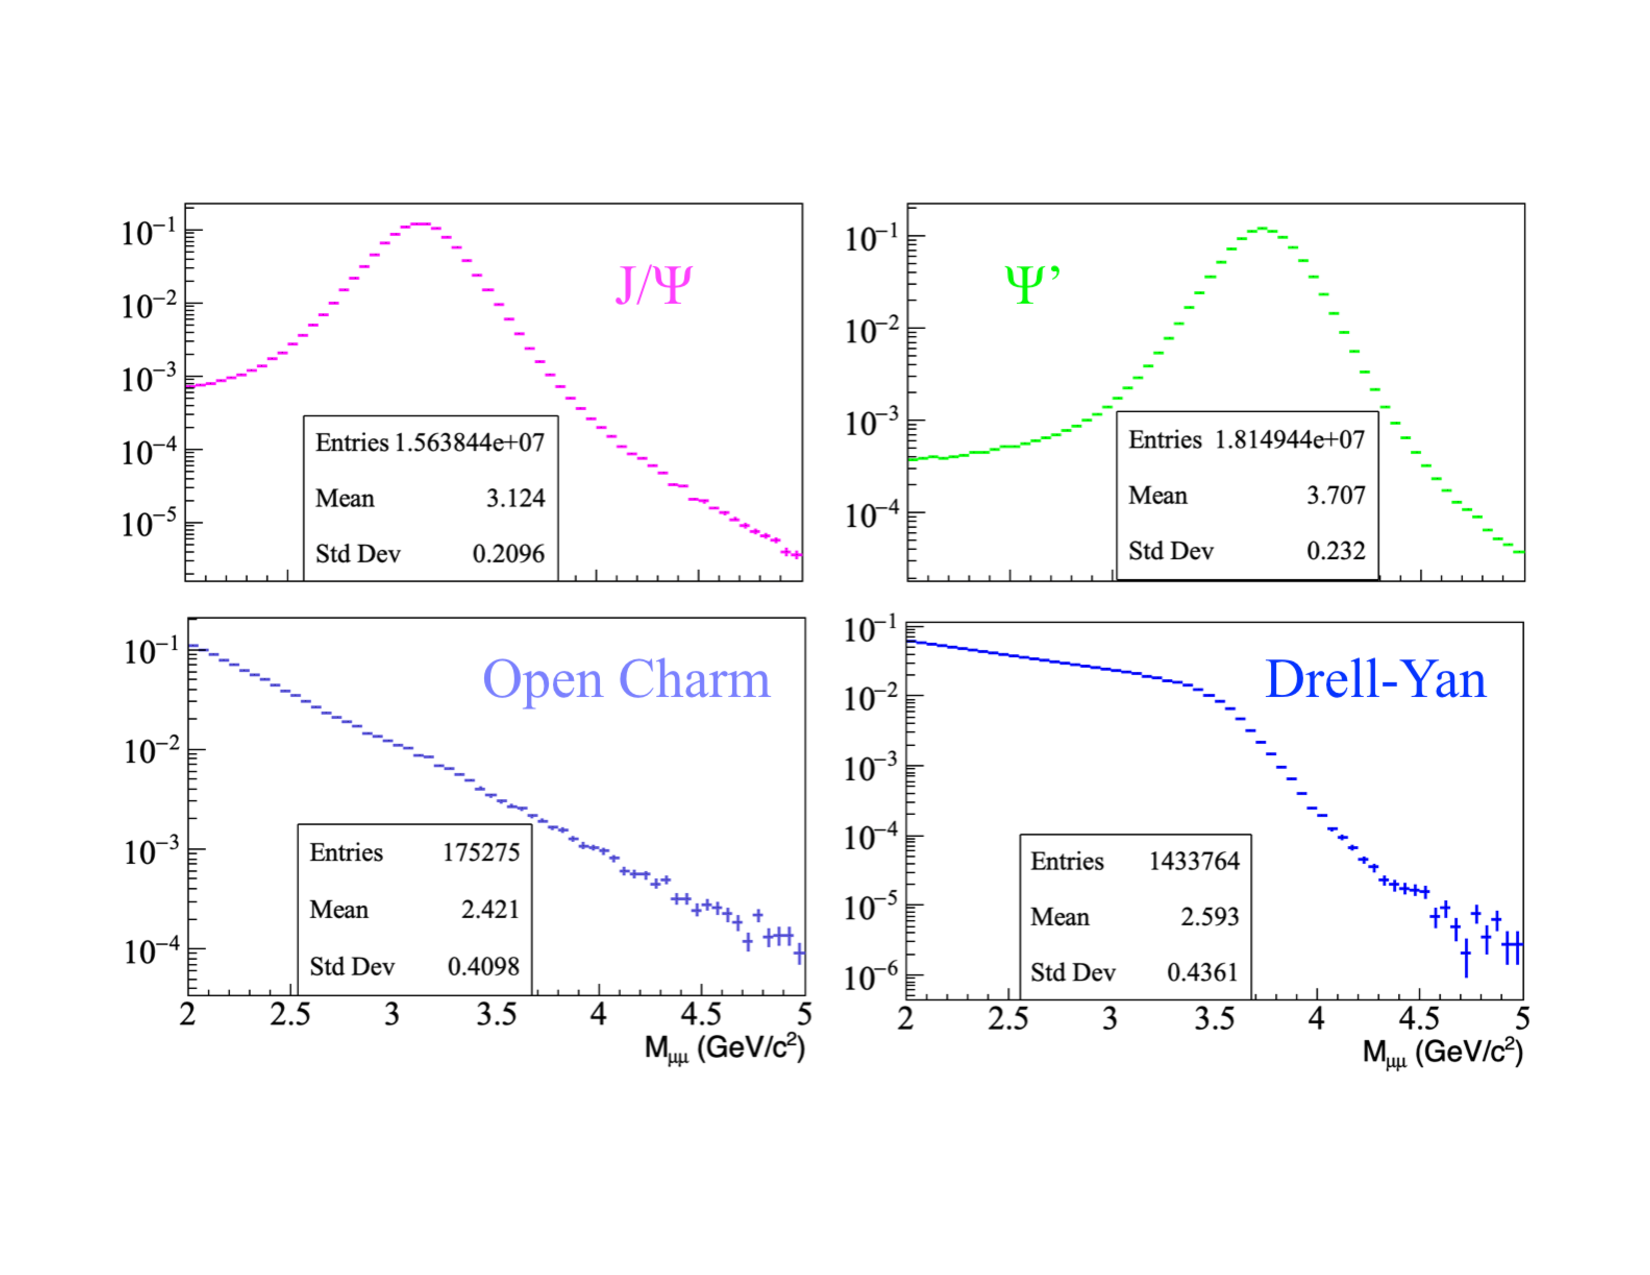
\includegraphics[width=0.8\textwidth, trim=2cm 3cm 2cm 3cm, clip]{MC_NormInvM}
  \caption{The normalized invariant mass distributions from the four simulated
    Monte-Carlo processes.  These distributions are used to fit the real data.}
  \label{fig::MC_NormInvM}
\end{figure}

\begin{figure}[h!t]
  \centering
  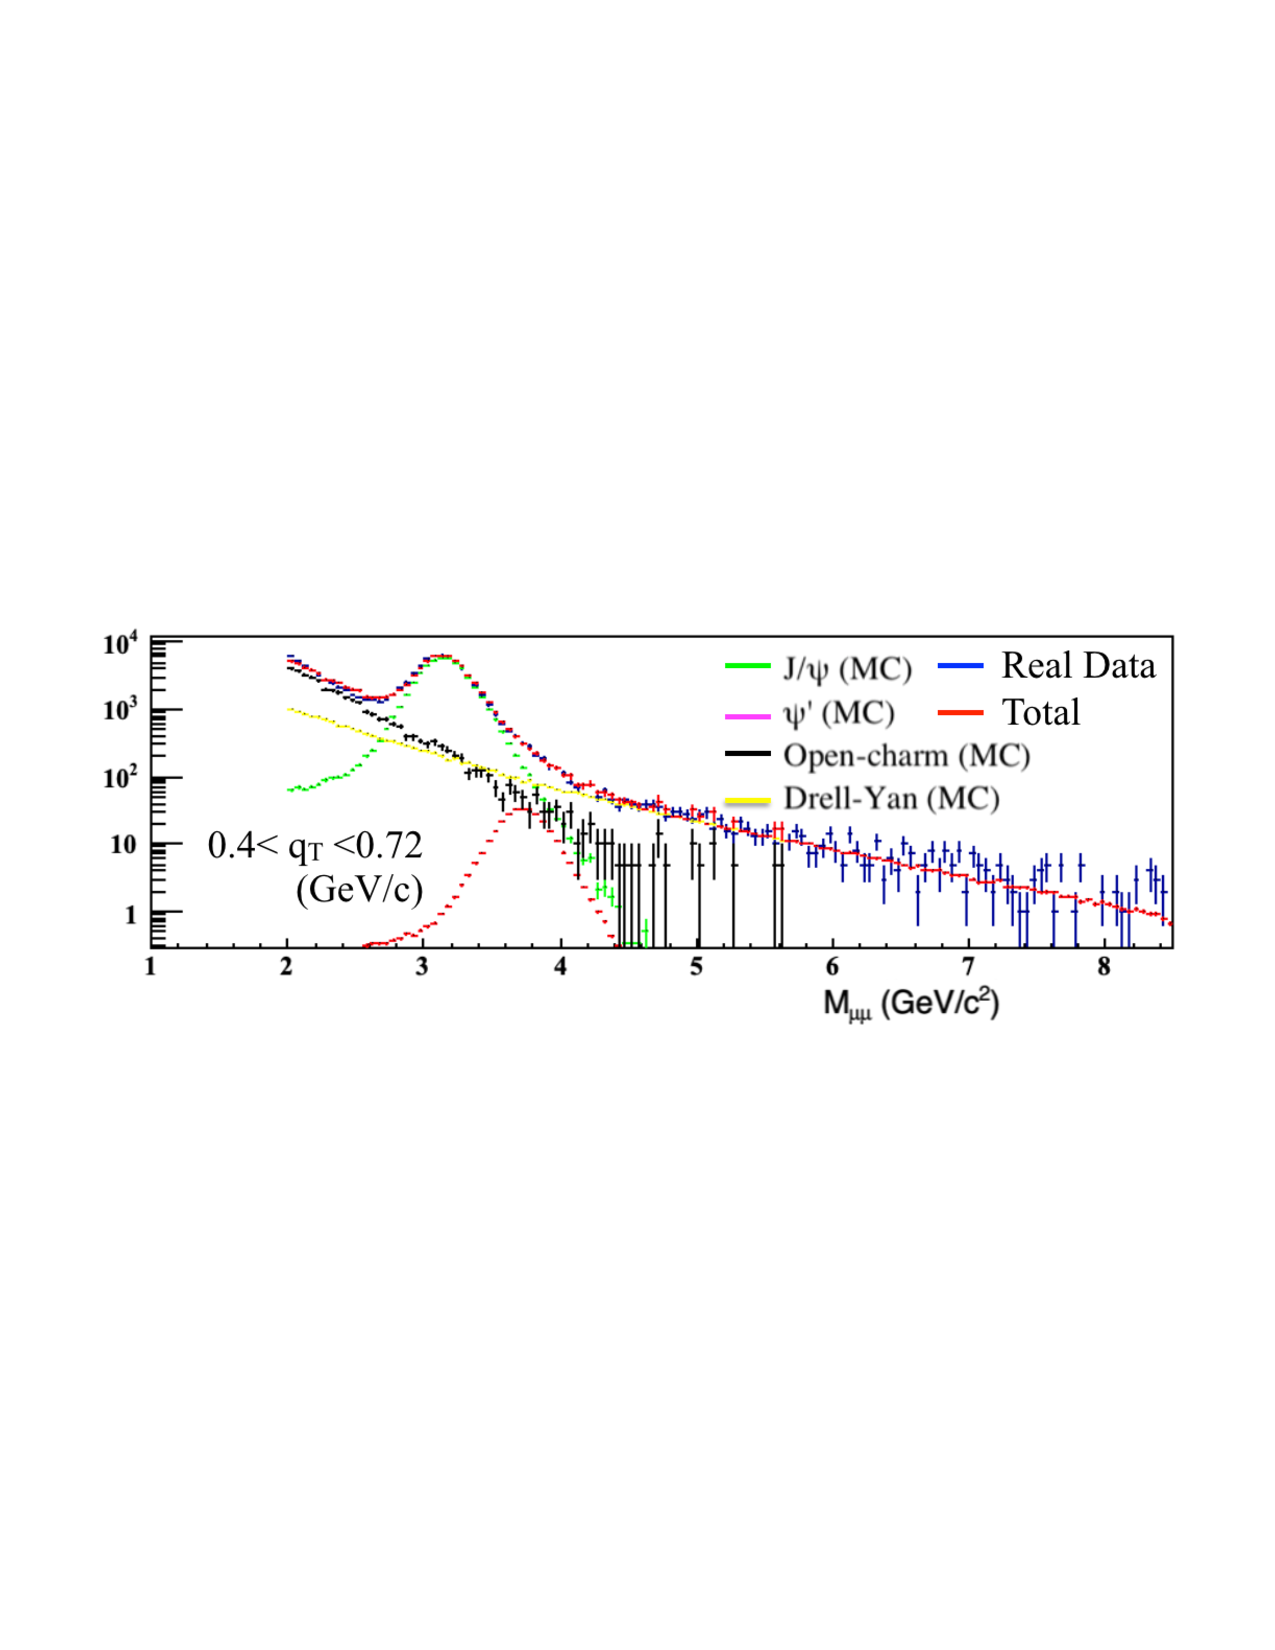
\includegraphics[width=0.8\textwidth, trim=1cm 10cm 1cm 10cm, clip]{MC_fitQt}
  \caption{}
  \label{fig::MC_fitQt}
\end{figure}

Once the fits are performed, the {\jp} purity in each invariant bin is
determined as

\begin{equation}
  p = \frac{N_{J/\Psi}}{N_{J/\Psi} + N_{Drell-Yan} + N_{Open\;Charm} +
    N_{\Psi'}}.
\end{equation}
\noindent
Table~\ref{tab::JPsiPurity} summarizes the {\jp} purity as a function of the
mass range.  For this analysis an invariant mass range of 2.87-3.38~{\gvcw} was
chosen to safely have a {\jp} purity of 90\% or greater.
Tables~\ref{tab::JPsiStats1}-~\ref{tab::JPsiStats2} summarizes the number of
events remaining after each cut.

\begin{table}
  \centering
  \begin{tabular}{ |c|c| }
    \hline
    \textbf{Mass range GeV/c$^2$}& \textbf{JPsi Purity \%}
    \\ \hline \hline
    2.5-4.3& 79.7 $\pm$ 2.9 \\ \hline
    2.78-3.46& 88.9 $\pm$ 2.0 \\ \hline
    2.87-3.38& 91.3 $\pm$ 1.5 \\ \hline
    2.95-3.29& 92.9 $\pm$ 1.0 \\ \hline
    3.08-3.17& 94.0 $\pm$ 1.0 \\ \hline
    
  \end{tabular}
  \caption{{\jp} purity}
  \label{tab::JPsiPurity}
\end{table}

\begin{table}[h!t]
  \begin{tabular}{ |c|c|c|c|c|c| }
    \hline \textbf{Cuts}& \textbf{W07}& \textbf{W08}& \textbf{W09}&
    \textbf{W10}& \textbf{W11} \\ \hline

    \multirow{3}{9em}{$\mu^-\mu^+$ 2-8.5 GeV/c$^2$ with a common best primary
      vertex}& & & & & \\
    & 1,573,372& 1,572,255& 1,620,593& 1,683,263& 2,598,485\\
    & & & & & \\ \hline
    
    Good Spills& 1,298,306& 1,223,877& 1,333,335& 1,374,620& 1,901,071
    \\ \hline
    
    0$<$ x$_{\pi}$ x$_N$ $<$1, -1$<$ x$_F$ $<$1& 1,298,278& 1,223,851&
    1,333,307& 1,374,599& 1,901,033 \\ \hline

    0.4$<$ q$_T$ $<$5(GeV/c)& 1,121,908& 1,056,835& 1,151,253& 1,187,125&
    1,641,463\\ \hline

    Z Vertex within NH$_3$& 314,965& 298,531& 324,413& 335,659& 465,172
    \\ \hline

    Vertex Radius $<$ 1.9cm& 308,278& 292,114& 317,985& 328,658& 455,580
    \\ \hline

    2.87$< M_{\mu\mu} <$3.38 (GeV/c$^2$)&
    170,041& 160,450& 174,696& 180,795& 250,921
    \\ \hline
    
  \end{tabular}
  \caption{Selected dimuon events for the first five data periods from the
    intermediate mass range analysis of 2015 COMPASS data}
  \label{tab::JPsiStats1}
\end{table}

\begin{table}[h!t]
  \begin{tabular}{ |c|c|c|c|c|c|c| }
    \hline \textbf{Cuts}& \textbf{W12}& \textbf{W13}& \textbf{W14}&
    \textbf{W15} & \textbf{WAll} & \textbf{Remaining} \\ \hline

    \multirow{3}{9em}{$\mu^-\mu^+$ 2-8.5 GeV/c$^2$ with a common best primary
      vertex}& & & & & & \\
    &1,932,425& 1,680,706& 1,094,525& 640,095& 14,395,719&
    100.00 \% \\ & & & & & & \\ \hline

    Good Spills& 1,659,030& 1,314,489& 982,131& 616,734& 11,703,593&
    81.3 \% \\ \hline

    0$<$ x$_{\pi}$ x$_N$ $<$1, -1$<$ x$_F$ $<$1&
    1,658,996& 1,314,470& 982,125& 616,720& 11,703,379&	81.3 \% \\ \hline

    0.4$<$ q$_T$ $<$5(GeV/c)&
    1,432,115& 1,134,223& 846,897& 532,045& 10,103,864&	70.2 \% \\ \hline

    Z Vertex within NH$_3$&
    406,975& 322,964& 241,673& 151,937&	2,862,289& 19.9  \% \\ \hline

    Vertex Radius $<$ 1.9cm&
    398,610& 316,149& 236,019& 148,834& 2,802,227& 19.5  \% \\ \hline

    2.87$< M_{\mu\mu} <$3.38 (GeV/c$^2$)&
    219,110& 173,701& 129,346& 81,808& 1,540,868& 10.7  \% \\ \hline
    
  \end{tabular}
  \caption{Selected dimuon events for the last four data periods and the total
    number of events from the intermediate mass range analysis of 2015 COMPASS
    data}
  \label{tab::JPsiStats2}
\end{table}


\subsection{Binning}

The analysis is determined as a function of the variables $x_N$, $x_{\pi}$,
$x_F$, $q_T$ and $M_{\mu\mu}$.  These are the same variables used to bin the
high mass Drell-Yan analysis.  The left-right asymmetry analysis is binned in
each of the kinematic variables by requiring an equal amount of data per
kinematic bin.  The bin limits are also required to have a width of at least
three times the resolution per variable.  For this analysis there is enough
statistics and the resolution per variable is good enough to have four kinematic
bins.  The bin limits are provided in Table~\ref{tab::JPsi_binning} and the
spectrometer resolutions are provided in Table~\ref{tab::JPsiRes}.

The spectrometer resolution is determined from the Monte-Carlo data.  The
resolution is determined from the difference between the Monte-Carlo generated
value and the reconstruction Monte-Carlo value.  An example of this distribution
is shown in Fig.~\ref{fig::JPsiXPiRes} for the $x_\pi$ variable.  The
distribution has a longer tail than a Gaussian distribution and for this reason
a two Gaussian fit function is used to determine the distributions width.  The
resolution is then determined as the width of the Gaussian with a larger
amplitude, so-called leading order Gaussian.  The actual spectrometer resolution
is between the width of the leading order Gaussian and the RMS of the
distribution.  However the leading order Gaussian width is closer to the true
resolution and is therefore used as the estimate for the spectrometer
resolution.

\begin{figure}[h!t]
  \centering
  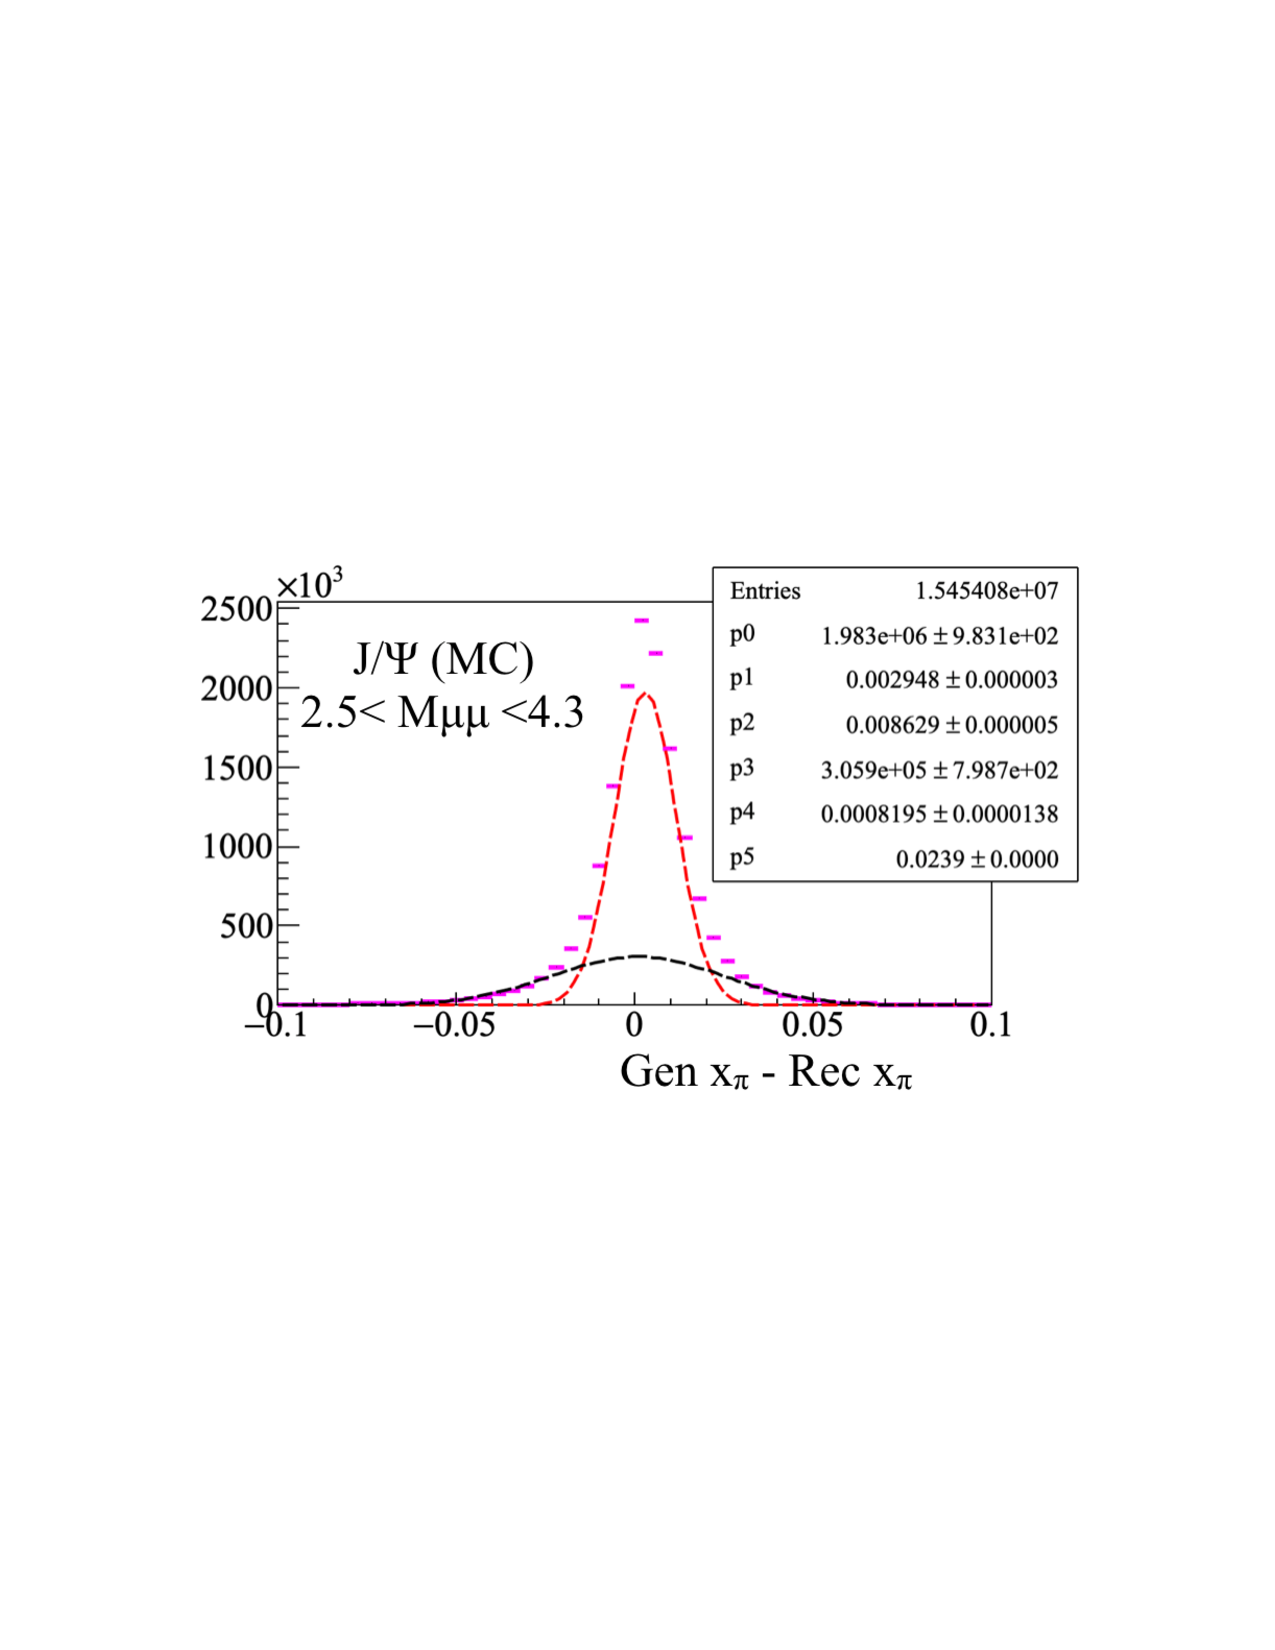
\includegraphics[width=0.6\textwidth, trim=3cm 9cm 3cm 9cm,clip]{JPsiXPiRes}
  \caption{The distribution of generated $x_N$ minus reconstructed $x_N$.  The
    leading Gaussian width (red) is used to determine the resolution.}
  \label{fig::JPsiXPiRes}
\end{figure}

\begin{table}[h!t]
  \centering
  \begin{tabular}{ |c|c|c| }
    \hline \textbf{Variable}& \textbf{RMS}& \textbf{Leading Gaussian $\sigma$}
    \\ \hline \hline
    
    $x_N$& 0.01& 0.006 \\ \hline

    $x_\pi$& 0.0157& 0.009 \\ \hline

    $x_F$& 0.016& 0.011 \\ \hline

    $q_T$& 0.143& 0.022 \\ \hline
  \end{tabular}
  \caption{The resolution in the intermediate mass range}
  \label{tab::JPsiRes}
\end{table}

\begin{table}[h!t]
  \begin{adjustwidth}{-1.4cm}{}
  \centering
  \begin{tabular}{ |c|c|c|c|c|c| }
    \hline \textbf{Variable}& \textbf{Lowest limit}& \textbf{Upper limit bin
      1}& \textbf{Upper limit bin 2}& \textbf{Upper limit bin 3}&
    \textbf{Upper limit bin 4}\\ \hline
    
    $x_N$& 0.0& 0.062& 0.083& 0.11& 1.0\\ \hline
    
    $x_{\pi}$& 0.0& 0.21& 0.28& 0.38& 1.0\\ \hline
    
    $x_F$& -1.0& 0.10& 0.20& 0.32& 1.0\\ \hline
    
    $q_T$ (GeV/c)& 0.4& 0.72& 1.04& 1.47& 5.0\\ \hline
    
    $M_{\mu\mu}$ (GeV/c$^2$)& 2.87& 3.03& 3.13& 3.22& 3.38 \\ \hline
    
  \end{tabular}
  \caption{{\jp} analysis bin limits}
  \label{tab::JPsi_binning}
  \end{adjustwidth}
\end{table}

The distributions for the binning variable shown in
Fig.~\ref{fig::JPsi_Kinematics}.  This analysis is performed in the valence
region for both the beam pion and target proton as the average $x_\pi$ is about
0.09 and the average $x_N$ is about 0.3.  This means the dominate contribution
to {\jp} production is from quark-quark interactions.  The average $q_T$ values
is below the minimum mass range of 2.87~{\gvcw} for this analysis and therefore
the interpretation of this analysis assumes the TMD regime is valid.

\begin{figure}[h!t]
  \centering 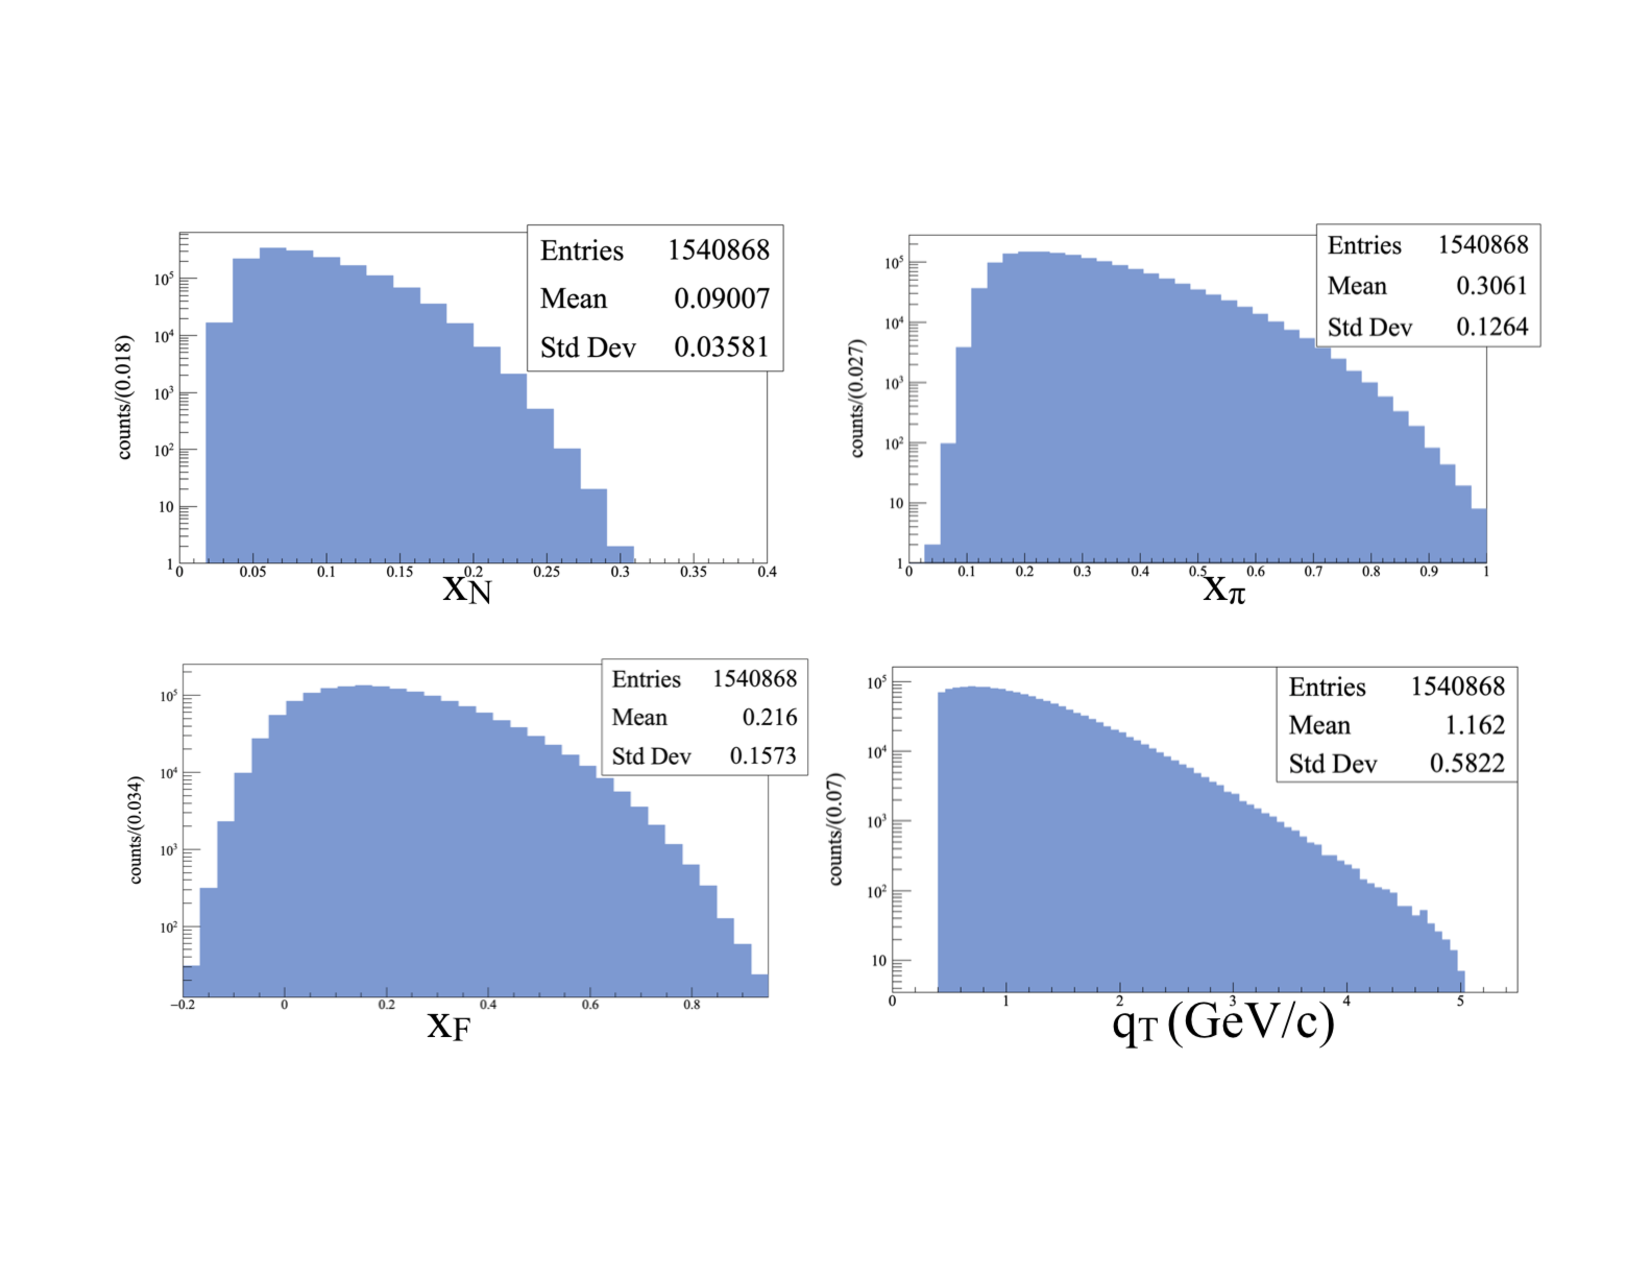
\includegraphics[width=0.95\textwidth,trim=1cm 3.5cm 1cm
    3.5cm,clip]{JPsi_Kinematics}
  \caption{The binning variable distributions. The longitudinal momentum
    fractions $x_N$ (top left) and $x_\pi$ (top right) and the $x_F$ (bottom
    left) and the virtual photon transverse momentum $q_T$ (bottom right).
    These distributions are in the mass range 2.87-3.38~{\gvcw}.}
  \label{fig::JPsi_Kinematics}
\end{figure}


\subsection{Asymmetry Extraction}
The asymmetry extraction method used is the two-target geometric mean.  This
asymmetry method is described in detail in
Secs~\ref{sec::leftrightasym}-~\ref{sec::TwoTargGeoMean}.  The asymmetry is
again defined as

\begin{equation}
  \label{equ::AN4TargGeomeanJPsi}
  A_{lr,2Targ} =
  \frac{1}{|S_T|}
  \frac{ \sqrt[4]{ N_{1,l}^\uparrow N_{1, l}^\downarrow
      N_{2,l}^\uparrow N_{2, l}^\downarrow }
    - \sqrt[4]{ N_{1,r}^\uparrow N_{1,r}^\downarrow
      N_{2,r}^\uparrow N_{2,r}^\downarrow }
  }{
    \sqrt[4]{ N_{1,l}^\uparrow N_{1, l}^\downarrow
      N_{2,l}^\uparrow N_{2, l}^\downarrow }
    + \sqrt[4]{ N_{1,r}^\uparrow N_{1,r}^\downarrow
      N_{2,r}^\uparrow N_{2,r}^\downarrow } },
\end{equation}
\noindent
where $N$ represents the counts, $l(r)$ denotes left(right), 1(2) denotes the
target cell and $\uparrow(\downarrow)$ denotes the transverse polarization
direction.  The definitions of left and right are defined relative to the target
spin as
\begin{equation}
  \begin{aligned}
    &\text{Left}: \hat{q}_T \cdot (\hat{S}_T \times \hat{P}_{\pi}) > 0 \\
    &\text{Right}: \hat{q}_T \cdot (\hat{S}_T \times \hat{P}_{\pi}) < 0, 
  \end{aligned}
\end{equation}
\noindent
where $\hat{q}_T$, $\hat{S}_T$ and $\hat{P}_{\pi}$ are unit vectors in the
target reference frame for the virtual photon transverse momentum, the target
spin and the beam pion momentum respectively.  The advantage to this asymmetry
method is that the acceptance from the upstream and downstream target cells
cancel as was shown in Eq.~\ref{equ::AN2targAcceptCancel}.  The statistical
uncertainty for this asymmetry method can be written as

\begin{equation}
  \delta A_{lr,2Targ} = \frac{1}{|S_T|}
  \frac{LR}{\Big( L+R \Big)^2}
  \sqrt{
    \sum_{c,p}
    \Big(
    \frac{1}{N_L^{p}}
    + \frac{1}{N_R^p}
    \Big)
  } \quad,
\end{equation}
where $L =\sqrt[4]{N_{1,L}^\uparrow N_{1,L}^\downarrow N_{2,L}^\uparrow
  N_{2,L}^\downarrow}$ and $R =\sqrt[4]{N_{1,R}^\uparrow N_{1,R}^\downarrow
  N_{2,R}^\uparrow N_{2,R}^\downarrow}$.  In the approximate case of equal
statistical populations in each left-right direction and each target cell, the
statistical uncertainty for the two-target geometric mean reduces to
$\frac{1}{|S_T|}\frac{1}{\sqrt{N}}$, where $N$ is the sum of all counts.

\subsection{Systematic Studies}

\subsection{Interpretation}

Doesn't fit anseminos plot...
